Vamos a ver como podemos utilizar algunas de las representaciones hasta ahora abordadas. Tomemos pues el siguiente problema de ejemplo:

\emph{Hacer un algoritmo que permita leer 2 números diferentes y nos diga cual es el mayor de los 2 números.}

\begin{figure}[!h]
	\centering
	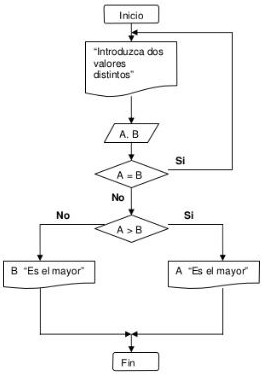
\includegraphics[width=0.35\linewidth]{img/ejemplo_diagrama-de_flujo_mayorymenor.jpg}
	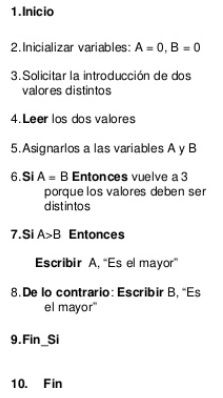
\includegraphics[width=0.3\linewidth]{img/pseudocodigo.jpg}
	\label{fig:diagramaflujo}
\end{figure}

Aquí hemos representado el algoritmo solución del mismo problema de la misma manera la izquierda por diagrama de flujo mientras a la derecha podemos observar el seudocódigo del mismo problema.